\section{Local Correlation}
\label{sec:3}
In this section, I introduce the term \textit{local correlation}, the base \textit{naive} approach, explain \textit{DFT-Based} algorithm for interactive pairwise correlation of subsequences of time-series data and show \textit{BRAID}, which is using an efficient principle of calculating the correlation coefficient.
\subsection{Foundations}
Correlation may occur in a burst, last for a particular duration, and then disappear. However, real data sets' signals often correlate with unknown lag. Intuitively, two signals have a local correlation with time delay $\tau$ if they look very similar when $\tau$ time ticks delay one signal. Without loss of generality, the data streams are sampled at a fixed rate, data are numeric, and all time-series are of the same length so that they can be treated as discrete signal sequences. It means that there are no missing timestamps. To simplify the problem and the algorithm's explanations, only one time-series has been lagged or shifted, and the correlation detection occurs only between two data streams. Still, it is possible to extend the detection to multiple time-series data streams ~\cite{ref18}. \newline

The numerical time-series data streams are denoted as $X$ and $Y$, so $x = \{x(0), \\x(1), \ldots, x(N- 1)\}$ stands for the subsequence of $X$ with limited length $N$, where $x(n) \in \mathbb{R}$ is the value of the $(n + 1)$-th data point of the subsequence. $len(x)$ is the length of $x$, and $st(x)$ is the starting time unit of $x$. Similar concepts are also applied to $Y$. Here, the correlation is evaluated by the widely applied Pearson correlation coefficient. Note that to compute the local correlation of $X$ and $Y$ with a time delay $\tau$, one time-series is first shifted by $\tau$ time ticks while keeping the other time-series fixed, and then the correlation is computed over their trimmed, common parts of length $(T - \tau)$, where $T$ is the maximum possible time delay. For two sequences $X$ and $Y$, which have the same length $N$ and time delay $\tau$, the Pearson correlation coefficient is calculated as:
\begin{equation}
\label{equ:6}
\begin{aligned}
r_{x y}(\tau)= & \frac{\sum_{n=0}^{N-\tau-1}\left(x_{n}-\bar{x}\right)\left(y_{n+\tau}-\bar{y}\right)}{\sqrt{\sum_{n=0}^{N-\tau-1}\left(x_{n}-\bar{x}\right)^{2}} \sqrt{\sum_{n=\tau}^{N-1}\left(y_{n}-\bar{y}\right)^{2}}}, \\\text{where}\quad&\bar{x}=\frac{1}{N-\tau}\sum_{n=0}^{N-\tau-1}x_{n},\quad\bar{y}=\frac{1}{N-\tau}\sum_{n=0}^{N-\tau-1}y_{n}
\end{aligned}
\end{equation}
Term $r_{x y}(\tau) \in[-1,1]$ indicates the linear correlation of the sequences and can reflect the similar behavior of sequence trend. Theoretically, when the evaluated parts of two sequences are correlated, $r_{x y}(\tau)$ will return a value close to $\mbox{1 or -1}$.

\subsection{Naive Solution}
The naive solution is the most apparent approach to finding and reporting correlated subsequences in a time-series data set. First, the approach starts with a single pair of time-series and picks subsequences from them. Then, for every possible time delay $\tau \in[-T, T],$ it calculates the Pearson correlation coefficient according to math equation \hyperref[equ:6]{(6)}. When it gets the Pearson correlation coefficients for all possible $\tau$ values in the predefined period, the maximal value is chosen as the Pearson correlation coefficient and the corresponding $\tau$. If the Pearson correlation coefficient exceeds the predefined threshold, it reports the correlation, and the related $\tau$ is returned as time delay. Note that to compute the local correlation of two time-series with a time delay $\tau$, one time-series is first shifted by $\tau$ time ticks while keeping the other time-series fixed. After processing the points in the current window, the current correlated subsequences should be saved if the correlation condition is satisfied. When the following data points come in, the Pearson correlation coefficient is calculated until the correlation is lost. Otherwise, the sliding window reads the following data points and recalculates the Pearson correlation coefficient. As a result, each pair decides correlation.\newline 

There is an advantage that it is pretty easy to implement, but also a disadvantage that for each new data point and each possible time delay, it is necessary to recalculate the correlation coefficient using the central math equation \hyperref[equ:6]{(6)}, which will result in high computation complexity. For the naive algorithm, the space complexity is $O(L + T)$, and the time complexity is $O(L * T)$, where $L$ is the length of the sliding window and $T$ is the maximal time delay.

\subsection{DFT-Based Solution~\cite{ref5}}
\begin{figure}[hb]
\centering
    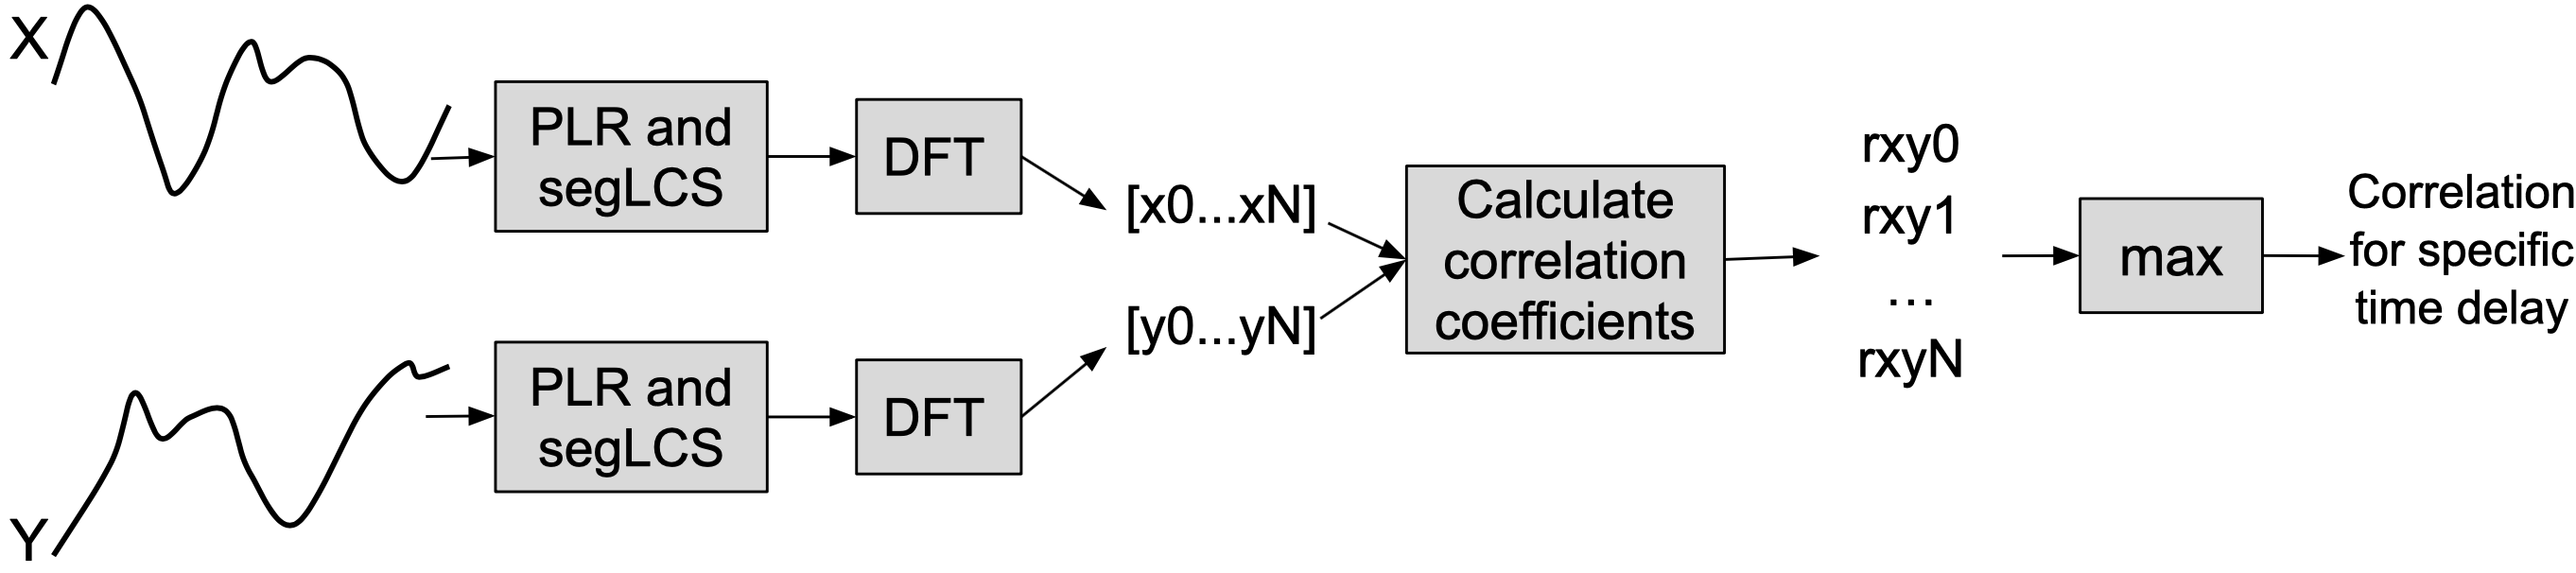
\includegraphics[width=\textwidth]{figures/dft.png}
    \caption{The DFT-Based Approach.}
    \label{fig:DFT}
\end{figure}
This solution is based on the advantage of the Discrete Fourier Transform (DFT) properties. It calculates the correlation coefficient with time delay by the inner product of normalized sequences of inverse Fourier Transform of two data stream sequences. The main algorithm order is the same as $naive$ but with another math logic calculation.\newline 

Now, I focus on the DFT foundation. Let $x=\{x(0), x(1), \ldots, x(n), \ldots, x(N-1)\}$ be a N-point sequence, and the \textit{Discrete Fourier Transform} of $x$ be $X=\{X(1)$, $X(2), \ldots, X(k), \ldots, X(N-1)\},$:
\begin{equation}
X(k)=\frac{1}{\sqrt{N}} \sum_{n=0}^{N-1} x(n) e^{-j \frac{2 \pi}{N} k n} \quad k \in[0, N-1]
\end{equation}
The inverse Fourier Transform of $X$ is
\begin{equation}
x(n)=\frac{1}{\sqrt{N}} \sum_{k=0}^{N-1} X(k) e^{j \frac{2 \pi}{N} k n} \quad n \in[0, N-1]
\end{equation}
If applying normalization to the sequence $x$, it is possible to generate the normalized sequence $\hat{x}$, where each sequence point value is
\begin{equation}
\hat{x}(n)=\frac{x(n)-\bar{x}}{\sqrt{\frac{1}{N} \sum(x(n)-\bar{x})^{2}}} \quad n \in[0, N-1]
\end{equation}
Similarly, it is possible also to normalize the N-point sequence $y$. The Pearson correlation coefficient of $x$ and $y$ can be calculated by the inner-product of normalized sequences $\hat{x}$ and $\hat{y}$:
\begin{equation}
r_{x y}(\tau)=\sum_{n=0}^{N-\tau-1} \hat{x}(n) \hat{y}(n+\tau)
\end{equation}
But the Pearson correlation function $r_{x y}(\tau)$ is directly calculated by inverse DFT on $R_{x y}$ after applying DFT on $\hat{x}$ and $\hat{y}$, because for two N-point sequences $x$ and $y$, if $r_{x y}(\tau)=\sum x(n) y(n+\tau),$ then the DFT of $r_{x y}(\tau)$ is given by $R_{x y}(k)=X^{*}(k) Y(k)$, where $X(k)$ and $Y(k)$ are the DFT of $x$ and $y$ respectively, and $X^{*}(k)$ denotes the complex conjugate of $X(k)$ and $\hat{X}(k)=\frac{X(k)}{\sqrt{\frac{1}{N} \sum(x(n)-\bar{x})^{2}}}$.~\cite{ref8} Since it is possible to derive the Pearson correlation coefficient with all possible time directly delay $\tau$, the computation complexity can be significantly improved. 
\begin{figure}[H]
\centering
    \label{fig:DFT_PLR}
    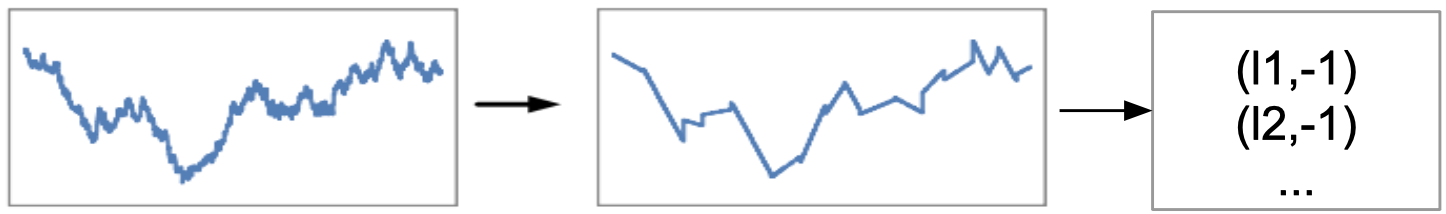
\includegraphics[width=0.8\textwidth]{figures/plr.png}
    \caption{The Piecewise Linear Representation and Segment trend sequence.}
\end{figure}
Now, I focus on the first step of this algorithm, utilizing linear representation to enhance the correlation detection, prune the correlation candidates, and help design efficient window sliding. Evaluating every new data point is a huge waste of time since there can be much redundancy. The authors defined piecewise linear representation for a data stream to reduce unnecessary calculations, make the window sliding more efficient, and accelerate the correlation analysis. It is to use line segments to approximate the data stream points continuously.~\cite{ref7} As shown in Figure \hyperref[fig:DFT_PLR]{4}, the data stream can be represented by several line segments, which can indicate the trend of the data stream. It leads to the following advantages: control of the approximation ratio and reduction in subsequence comparisons because the sliding procedure can go ahead segment by segment rather than point by point. Also, piecewise linear representation can prune the unnecessary calculation from an early stage. \newline 

Since the correlation is sensitive to the increasing and decreasing trend of data point values, the next step is an evaluation of the similarity of line segments from the view of data-changing trends. After generating line segments, it transfers the line segments into pairs of numbers. Each segment pair describes a line segment's characteristics, consisting of the length of the line segment and the changing trend. If the slope of the line segment is greater than 0, then the changing trend is 1; otherwise, the changing trend is -1. For example in Figure \hyperref[fig:DFT_PLR]{4}, $\{(l_{1},-1),(l_{2},-1)\}$ means the sequence is approximated by two segments. The first one has $l_{1}$ points and is decreasing; the length of the second one is $l_{2}$, and it is also decreasing. So, for the two subsequences in the sliding window, it is possible first to compare their similarity by the segment trend sequences. If two sequences are in correlation, their segment trend sequences should be similar since the correlation indicates the linear dependency of the sequences. If the two trend sequences are similar enough, the approach continues on the local correlation evaluation; otherwise, the sliding window moves on to receive new coming points. \newline

There are three advantages: The Discrete Fourier Transform allows rapid correlation calculation with time delay — 30\% reduction of running time. Based on the properties of the approximation technique, it is possible to make early pruning to avoid unnecessary calculations by estimating the correlation. Additionally, it reduces running time because it only concerns the XOR operation for similarity of line segments analysis. On the other hand, there are a lot of redundant evaluations of every new data point. For the DFT-based algorithm, the space complexity is $O(L)$, and the time complexity is $O(L * log(L))$, where $L$ is the length of the sliding window.
\subsubsection{Evaluation}
The authors test the algorithm on synthetic and real data streams so that the conclusion can be made based on a wide range of data distribution. For real data, they have chosen the Sunspots\footnote{\href{ftp://ftp.ngdc.noaa.gov/STP/SOLAR_DATA/SUNSPOT_NUMBERS/}{ftp://ftp.ngdc.noaa.gov/stp/solar\_data/sunspot\_numbers/}} and Temperature\footnote{\href{http://lwf.ncdc.noaa.gov/oa/climate/ research/anomalies/index.html}{http://lwf.ncdc.noaa.gov/oa/climate/ research/anomalies/index.html}} data sets. Sunspots consist of the data set that describes the daily sunspot numbers from 01.01.1945 to 31.10.2009 with 23680 records. It randomly extracted two subsequences from the 23680 records as two data streams, each comprising around 1800 data points. Temperature consists of monthly data records measuring the land and ocean temperatures as data streams. Each of the streams consists of 1560 data points. The correlation between them indicates the link between land temperature and ocean temperature. \newline

The authors found that the results detected by the DFT-based algorithm are mainly laid on the correlation score curve of the naive algorithm at the occurrence of correlation, demonstrating this solution's effectiveness. The DFT-Based algorithm can detect most of the correlation and effectively reduce the false alarm on the subsequences with low visual similarity. When the maximal time delay is slight, the running time of the DFT-Based algorithm is longer than the naive solution because the DFT-Based algorithm continuously calculates the Pearson correlation coefficient with every possible time delay, even if it exceeds $T$. However, with the growth of $T$, the DFT-Based algorithm significantly outperforms the naive algorithm, bringing improvement at about 80\% off. Finally, the random data set test showed an impressive pruning rate of 95\% at least. 

\subsection{BRAID Solution~\cite{ref6}}
\begin{figure}[hb]
\centering
    \label{fig:BRAID}
    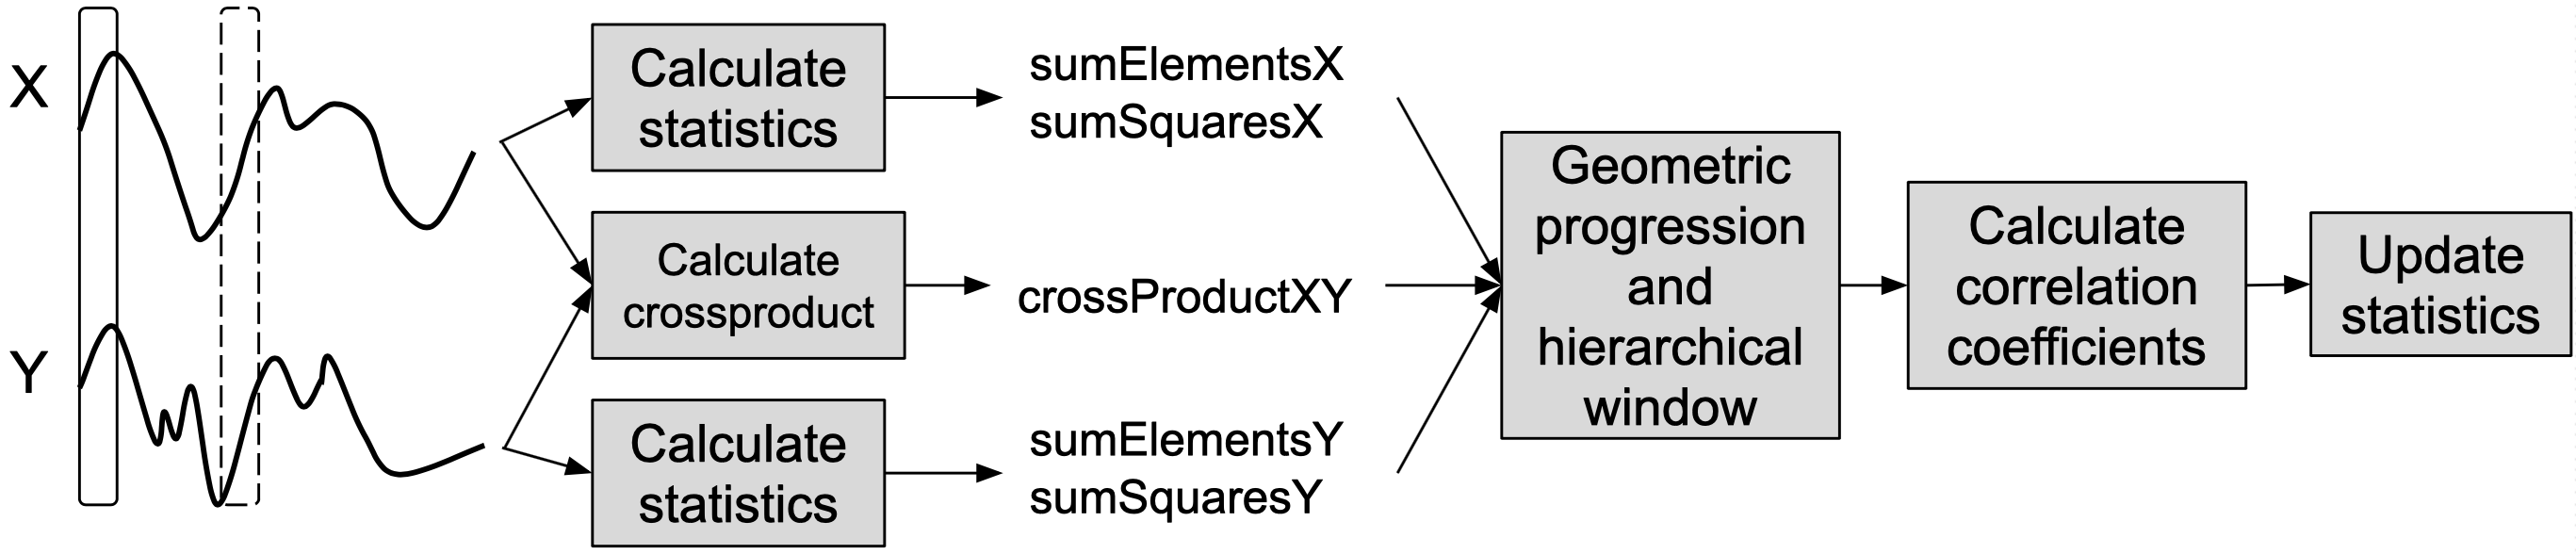
\includegraphics[width=\textwidth]{figures/braid.png}
    \caption{The BRAID approach.}
\end{figure}
In section \hyperref[sec:iBRAID]{2.3}, I have already described that the BRAID solution is based on the hypothesis that interactivity can be achieved by integrating caching. This algorithm technique partially solved the problem of the naive approach by efficiently and incrementally calculating the Pearson correlation coefficient based on five basic and computationally cheap sufficient statistics. However, linear time is still needed to compute the Pearson correlation function between the two time-series. \newline

The authors introduced an approximation using a geometrical progression to reduce the lag-estimation time. In other words, instead of computing correlation coefficients for every possible period value, it is necessary to track only the geometric progression of the period values with step 2 ($\tau = 0,1,2,4, \ldots, 2^{i}$). It means that only $O(log(n))$ numbers are necessary to estimate the Pearson correlation function, instead of $O(n)$ that the naive solution requires. Of course, this approximation introduces error. \newline

This method will give good accuracy for small $\tau$ precisely because for small $\ tau$'s, there are many points to interpolate. It may provide a larger error for large delay $\tau$, but the relative error will probably be small. But the space required grows linearly with the length $n$ because for computation of the Pearson correlation coefficients at any time $\tau$, it is necessary to keep a sliding window of size $l$ ($O(n)$ space required). So, the authors introduced the smoothed version of sequences to estimate the Pearson correlation function. It means $O(log(n))$ space and $O(1)$ time by the geometric probing and sequence smoothing.
\begin{figure}[H]
\centering
    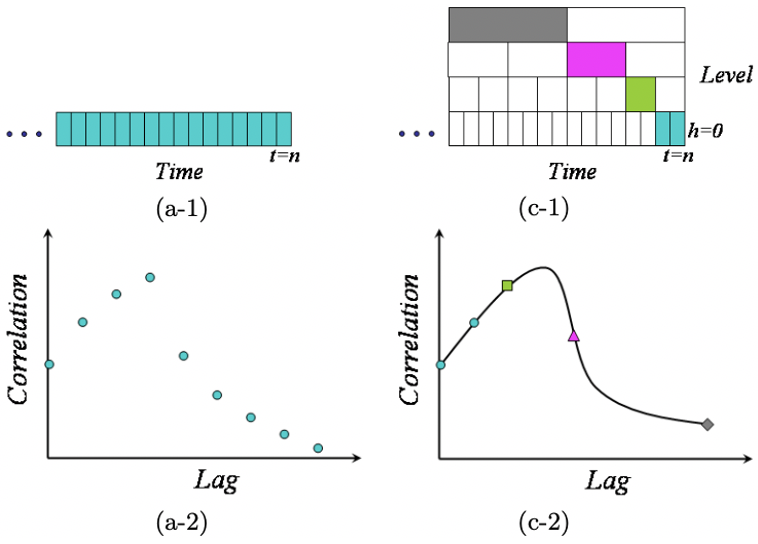
\includegraphics[width=0.55\textwidth]{figures/1.png}
    \caption{Hierarchical windowing and cubic spline interpolation.}
    \label{fig:BRAID_graphs}
\end{figure}
Instead of operating on the original time sequences, the approach computes their smoothed version by adding non-overlapping windows. The window widths will be powers of 2, although any other number would also be acceptable. Figure \hyperref[fig:BRAID_graphs]{6} (a) illustrates the naive approach: Figure \hyperref[fig:BRAID_graphs]{6} (a-1) denotes that the values for all the time delays are kept. Figure \hyperref[fig:BRAID_graphs]{6} (a-2) shows an illustration of the Pearson correlation function for two subsequences. Figure \hyperref[fig:BRAID_graphs]{6} (c) offers the BRAID solution. The redundant points were eliminated here, favoring the smallest window, which should give more accurate results. Figure \hyperref[fig:BRAID_graphs]{6} (c-2) shows the correlation coefficients obtained from the selected window averages shown in Figure \hyperref[fig:BRAID_graphs]{6} (c-1). The colored boxes represent BRAID's window averages for computing correlation coefficients and capturing time delay. BRAID ignores the white ones and does not calculate their window averages. It computes window averages for every level and correlation coefficients for several time delays incrementally. The missing Pearson correlation coefficients caused by the approximation are estimated by interpolation with a cubic spline. Firstly, there are nine blue points. Next, only 0, 1, 2, 4, and 8 points are chosen. As a result, an off-the-shelf interpolation method was used to obtain a smoother curve to find the local maximum of the Pearson correlation function (Brent's method~\cite{ref17}).
\subsubsection{Evaluation}
The authors test the algorithm on synthetic and real data streams so that the conclusion can be made based on a wide range of data distribution. For real data, they have chosen humidity, height, and temperature readings, Kursk and Sunspots\footnote{\href{http://csep10.phys.utk.edu/astr162/lect/sun/sscycle.html}{http://csep10.phys.utk.edu/astr162/lect/sun/sscycle.html}}. Humidity, Light, Temperature consist of humidity, illuminance, and temperature readings, from 55 sensors within several buildings. Each sensor gives a reading every 30 seconds. The authors have chosen two sequences for each data set, humidity and light, and used all sequences for temperature. Kursk consists of seismic recordings from multiple sensors, showing the Russian submarine "Kursk" explosion. Each sequence has a single burst. The authors extracted two subsequences of length n=70,000. Sunspots consist of several sunspots per day. The data set has a period of approximately 11 years. The authors have chosen two intervals from the data set, each length n=25,900, and treated them as two different time sequences.\newline

The results show that BRAID ideally approximates the Pearson correlation coefficients of the sinusoidal wave. Also, they indicate that BRAID closely estimates the Pearson correlation coefficients using interpolation and captures the local correlations of the spike. The experiments demonstrate that BRAID detects the correct time delay perfectly most of the time. The most significant relative error was about 1\%. Instead of the $O(n)$ that the naive implementation requires, BRAID can dramatically reduce computation time. Theoretically, BRAID requires time $O(1)$ for updating the sufficient statistics; the computation time does not depend on $n$. In this experiment, the time increases slightly as $n$ grows. This increase is caused by interpolation through a more significant $O(log(n))$ number of points. Specifically, BRAID is up to about 40,000 times faster than the naive implementation.